\section{Generative Models for Video \& Images}
\begin{frame}{}
    \LARGE Video Learning \& Generation: \textbf{Generative Models for Video \& Images}
\end{frame}

\begin{frame}{Generative Models for Video \& Images}
    \begin{itemize}
        \item Generative models learn to generate new data samples that resemble the training data.
        \item They can be used for tasks like image synthesis, video generation, and style transfer.
        \item Common approaches include Generative Adversarial Networks (GANs), Variational Autoencoders (VAEs), and diffusion models.
    \end{itemize}
\end{frame}

\subsection{VQ-GAN – Vector Quantized Generative Adversarial Network}
\begin{frame}[allowframebreaks]{VQ-GAN}
    \large VQ-GAN – Vector Quantized Generative Adversarial Network \\[1em]
    \textbf{VQ-GAN} is a generative model that combines the strengths of vector quantization and GANs to generate high-quality images.

    \begin{itemize}
        \item \textbf{Vector Quantization:} Encodes images into discrete latent codes, allowing for efficient representation and generation.
        \item \textbf{GAN Framework:} Uses a discriminator to guide the generator in producing realistic images.
        \item \textbf{Applications:} Image synthesis, super-resolution, and style transfer.
    \end{itemize}
\framebreak
    \textbf{Architecture:} VQ-GAN consists of an encoder, a quantizer, a decoder, and a discriminator.
    \begin{itemize}
        \item \textbf{Encoder:} Maps input images to a continuous latent space.
        \item \textbf{Quantizer:} Discretizes the continuous latent space into a finite set of codes.
        \item \textbf{Decoder:} Reconstructs images from the quantized latent codes.
        \item \textbf{Discriminator:} Evaluates the realism of generated images, providing feedback to the generator.
    \end{itemize}
\framebreak
    \begin{figure}
        \centering
        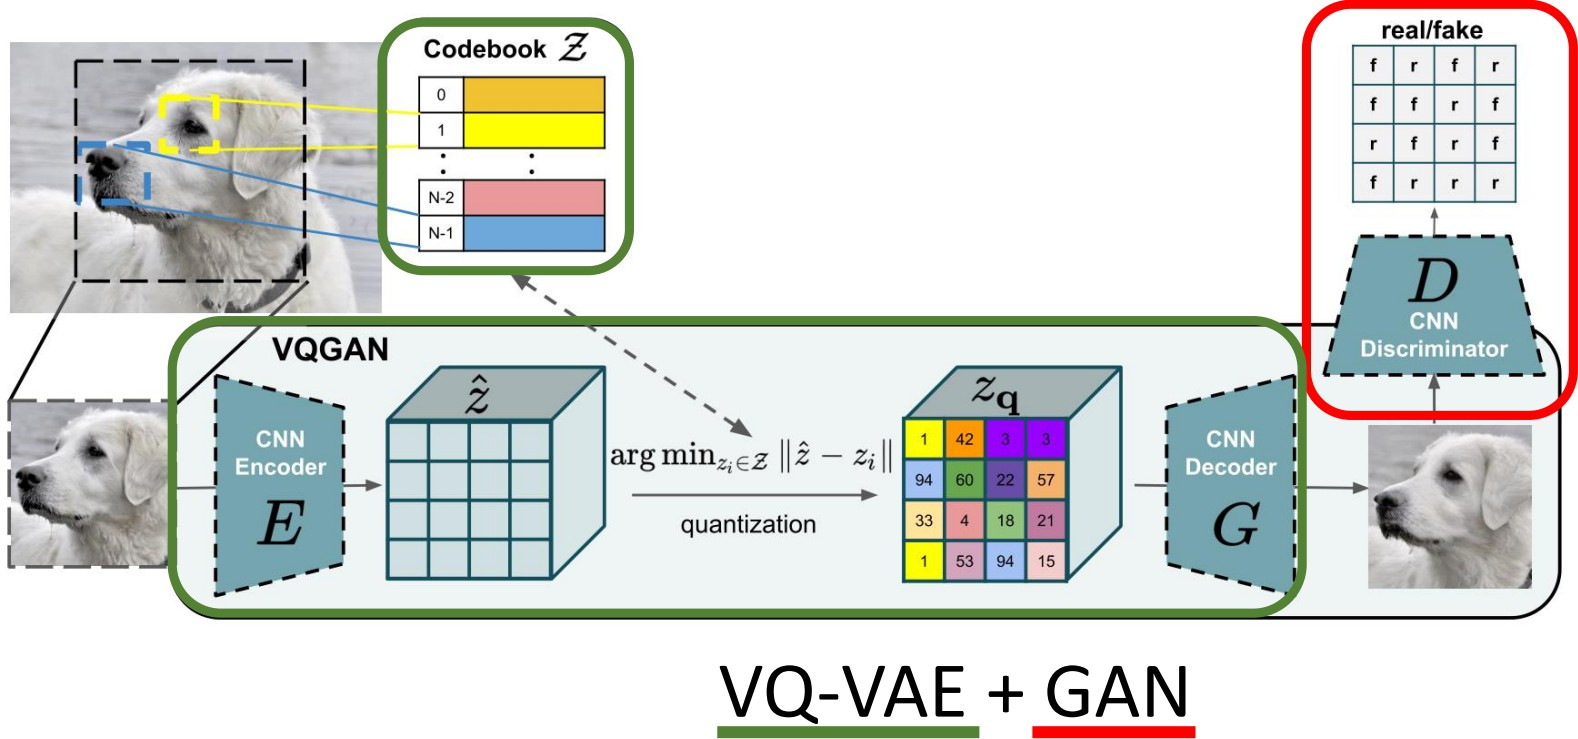
\includegraphics[width=1\textwidth,height=0.9\textheight,keepaspectratio]{images/video/slide_59_1_img.jpg}
    \end{figure}
\end{frame}

\subsection{VQ-GAN + CLIP}
\begin{frame}[allowframebreaks]{VQ-GAN + CLIP}
    \large
    \textbf{VQ-GAN + CLIP} is a powerful combination of two models that enhances image generation and understanding by leveraging the strengths of both vector quantization and contrastive learning.

    \begin{itemize}
        \item \textbf{VQ-GAN:} A generative model that uses vector quantization to encode images into discrete latent codes, enabling efficient representation and high-quality image synthesis.
        \item \textbf{CLIP:} A model that learns visual representations by aligning images and text, allowing for zero-shot classification and improved understanding of visual content.
    \end{itemize}
\framebreak
    \textbf{How They Work Together:}
    \begin{itemize}
        \item \textbf{Image Generation:} VQ-GAN generates images by decoding quantized latent codes, while CLIP provides a text-based conditioning mechanism that guides the generation process.
        \item \textbf{Text Conditioning:} CLIP's text embeddings can be used to condition the VQ-GAN generator, allowing it to produce images that match specific textual descriptions.
        \item \textbf{Loss Function:} The similarity between generated image embeddings and text embeddings from CLIP can be used as a loss function to optimize the VQ-GAN generator, ensuring that the generated images align with the given text prompts.
    \end{itemize}
\framebreak
    \begin{figure}
        \centering
        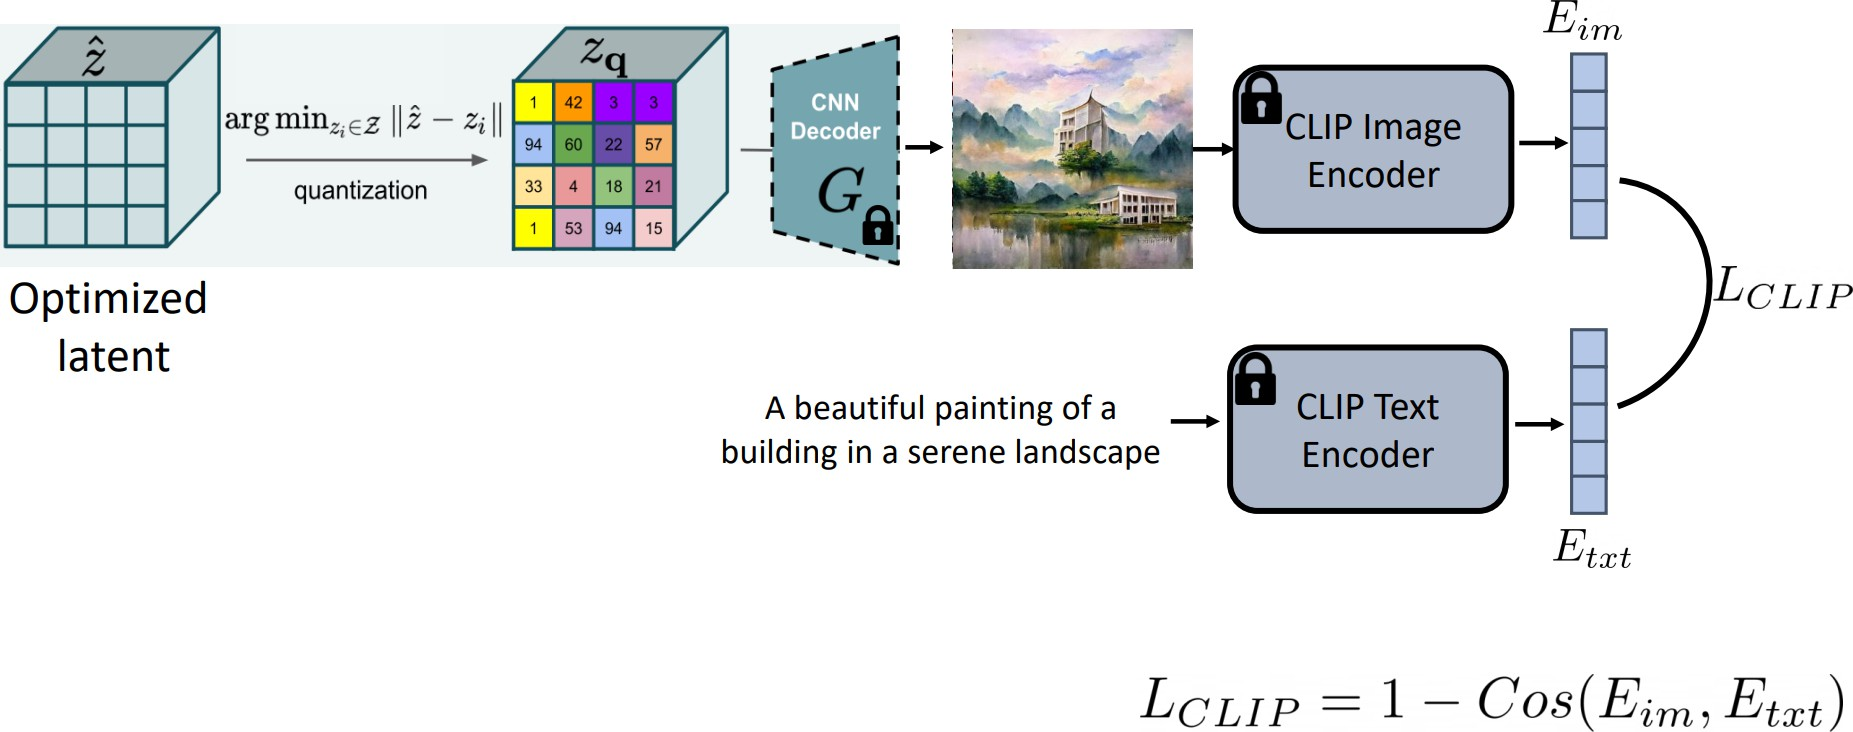
\includegraphics[width=1\textwidth,height=0.8\textheight,keepaspectratio]{images/video/slide_60_1_img.jpg}
    \end{figure}
    {\footnotesize{[VQGAN-CLIP: Open Domain Image Generation and Editing with Natural Language Guidance, Crowson et al. ICCV 13 2021]}}

\framebreak
    \large
    \textbf{Applications:}
    \begin{itemize}
        \item \textbf{Text-to-Image Synthesis:} VQ-GAN + CLIP can generate images based on textual descriptions, enabling creative applications like art generation and design.
        \item \textbf{Image Editing:} The combination allows for editing images based on text prompts, such as changing the style or content of an image while preserving its structure.
        \item \textbf{Zero-Shot Learning:} CLIP's zero-shot capabilities can be leveraged to classify generated images into categories without additional training, enhancing the versatility of the model.
    \end{itemize}

\framebreak
    \begin{figure}
        \centering
        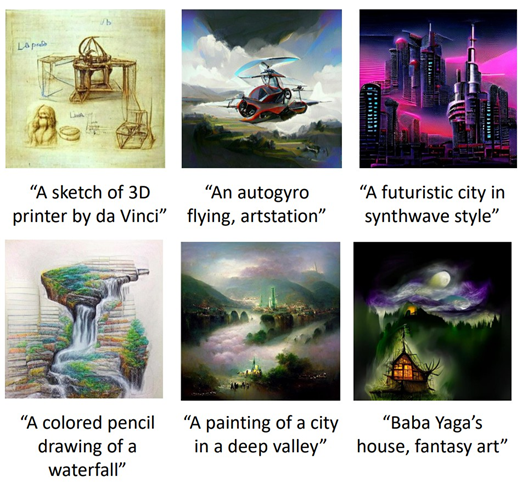
\includegraphics[width=1\textwidth,height=0.9\textheight,keepaspectratio]{images/video/slide_61_1_img.png}
    \end{figure}
\end{frame}
\subsection{VQ-GAN + CLIP Editing}
\begin{frame}[allowframebreaks]{Using CLIP for generative tasks}
    \begin{figure}
        \centering
        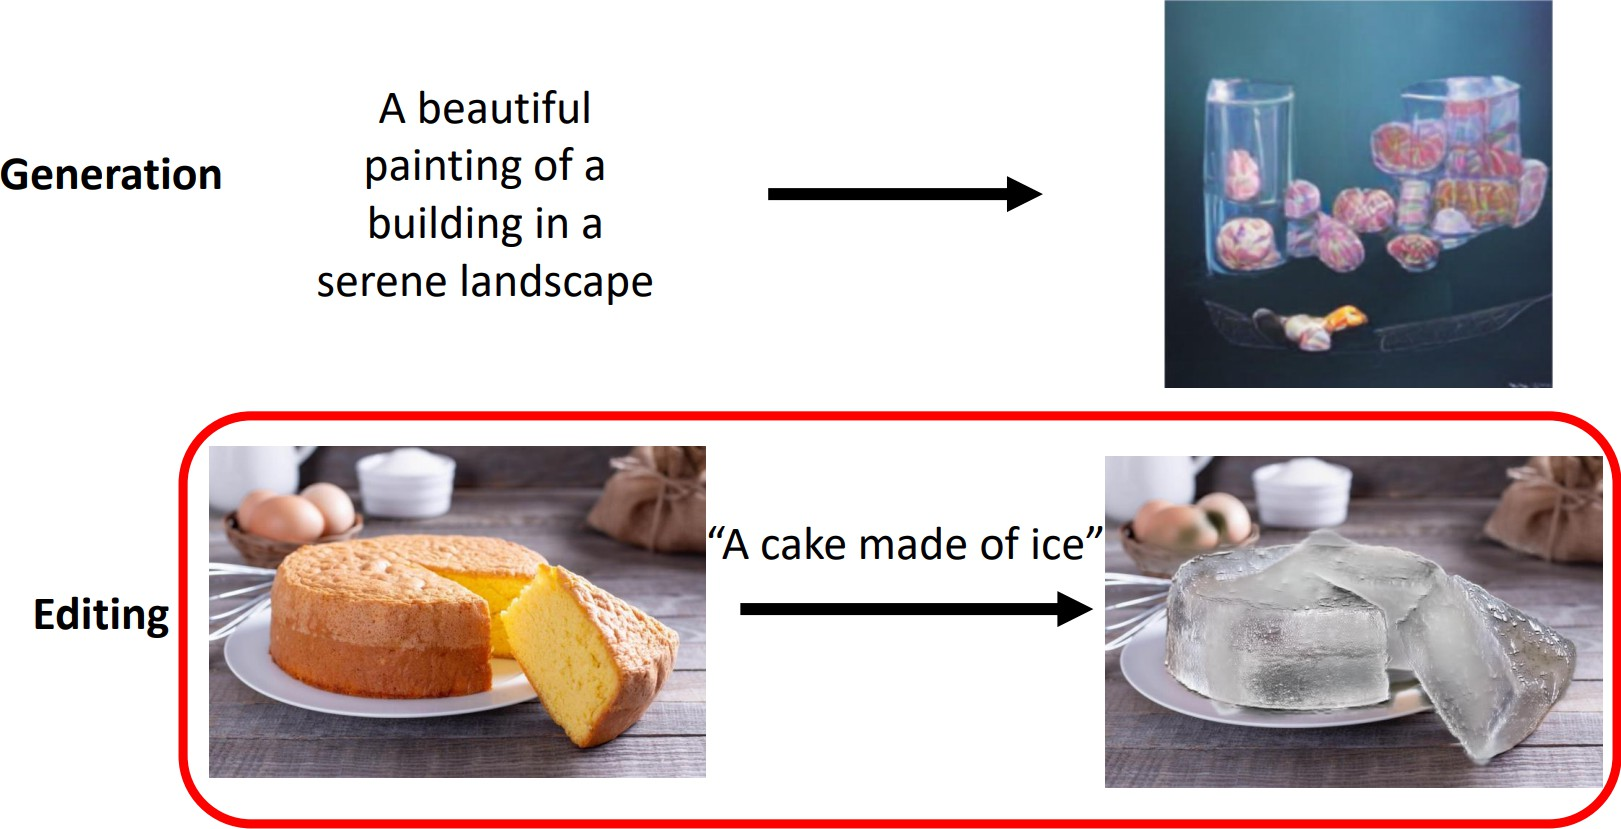
\includegraphics[width=1\textwidth,height=0.9\textheight,keepaspectratio]{images/video/slide_62_1_img.jpg}
    \end{figure}
\end{frame}


\begin{frame}[allowframebreaks]{VQ-GAN + CLIP Editing}
    \large VQ-GAN + CLIP Editing \\[1em]
    \textbf{VQ-GAN + CLIP Editing} combines the strengths of VQ-GAN for image generation and CLIP for text-guided editing, enabling high-quality image synthesis and manipulation.

    \begin{itemize}
        \item \textbf{VQ-GAN:} Generates images from discrete latent codes, allowing for efficient representation.
        \item \textbf{CLIP:} Guides the editing process by understanding text prompts, enabling targeted modifications to generated images.
        \item \textbf{Applications:} Image synthesis, style transfer, and content-aware editing.
    \end{itemize}
\framebreak
    \textbf{How They Work Together:}
    \begin{itemize}
        \item \textbf{Image Generation:} VQ-GAN generates images based on quantized latent codes, while CLIP provides text-based guidance for editing.
        \item \textbf{Text Conditioning:} CLIP's text embeddings condition the VQ-GAN generator, allowing it to produce images that match specific textual descriptions.
        \item \textbf{Loss Function:} The similarity between generated image embeddings and text embeddings from CLIP is used as a loss function to optimize the VQ-GAN generator, ensuring that the generated images align with the given text prompts.
    \end{itemize}
\framebreak
    \begin{figure}
        \centering
        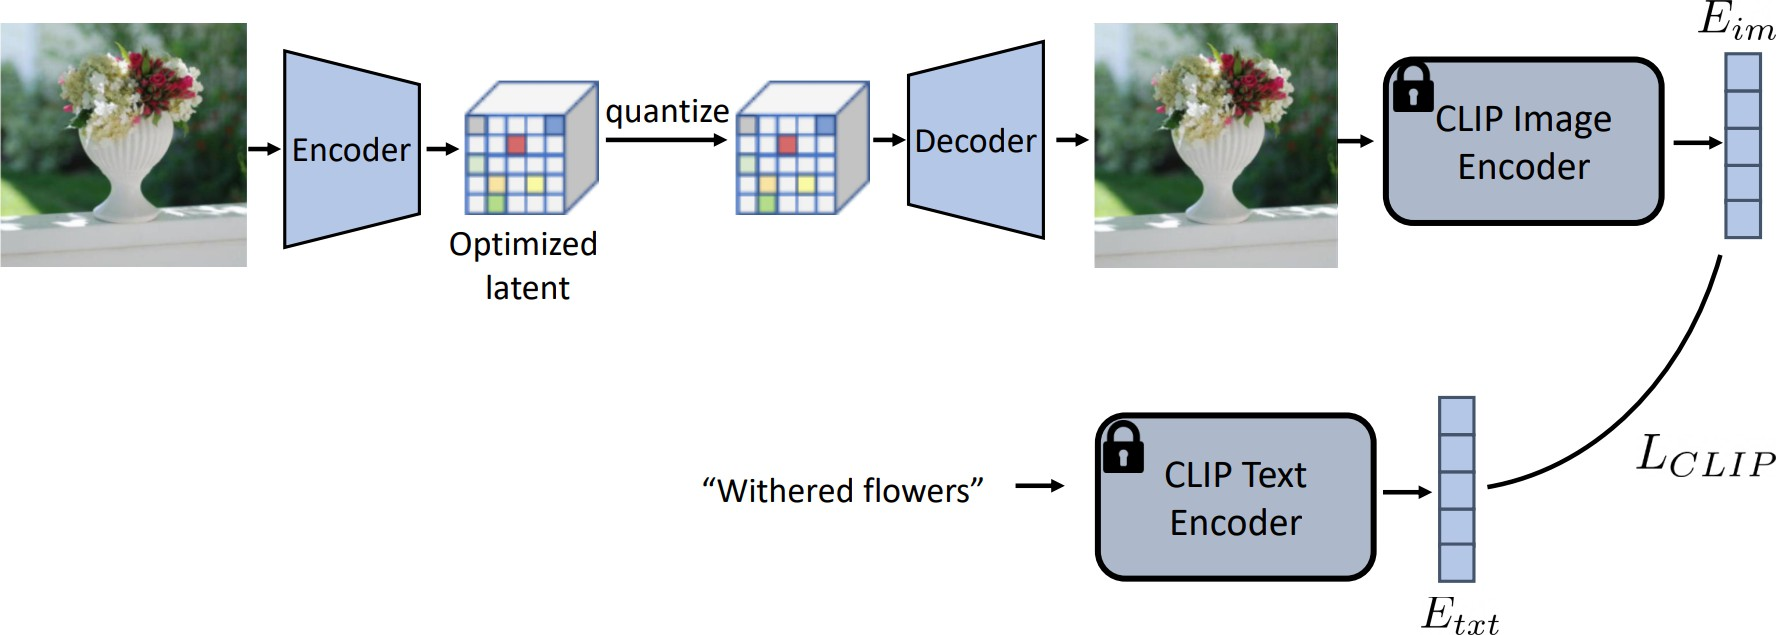
\includegraphics[width=1\textwidth,height=0.8\textheight,keepaspectratio]{images/video/slide_63_1_img.jpg}
    \end{figure}
    {\footnotesize{[VQGAN-CLIP: Open Domain Image Generation and Editing with Natural Language Guidance, Crowson et al. ICCV 13 2021]}}
\framebreak
    \begin{figure}
        \centering
        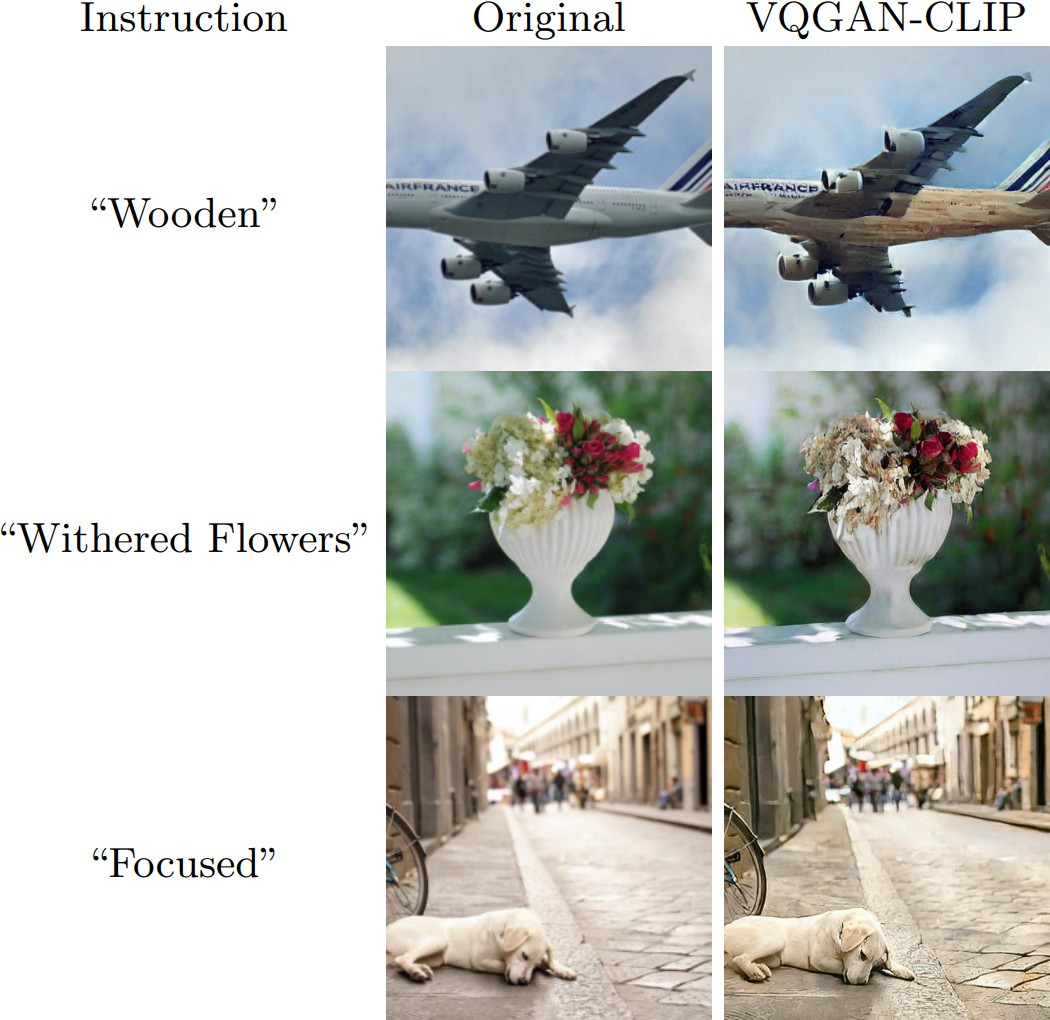
\includegraphics[width=1\textwidth,height=0.9\textheight,keepaspectratio]{images/video/slide_64_1_img.jpg}
    \end{figure}
\end{frame}
\subsection{StyleCLIP}
\begin{frame}[allowframebreaks]{StyleCLIP}
    \textbf{StyleCLIP} is a method that combines the power of CLIP (Contrastive Language-Image Pretraining) with StyleGAN to generate images based on text prompts, allowing for fine-grained control over image attributes.

    \begin{itemize}
        \item \textbf{CLIP Embeddings:} Uses CLIP to encode text prompts into embeddings that capture semantic information.
        \item \textbf{StyleGAN Manipulation:} Applies these embeddings to manipulate the latent space of StyleGAN, enabling the generation of images that match the desired attributes described in the text.
        \item \textbf{Applications:} Useful for tasks like image editing, attribute manipulation, and creative content generation.
        \item \textbf{Benefits:} Provides a powerful way to generate diverse images based on textual descriptions.
        \item \textbf{Costs:} Requires careful tuning of the StyleGAN latent space and may produce artifacts if not managed properly.
    \end{itemize}
\framebreak
    \begin{figure}
        \centering
        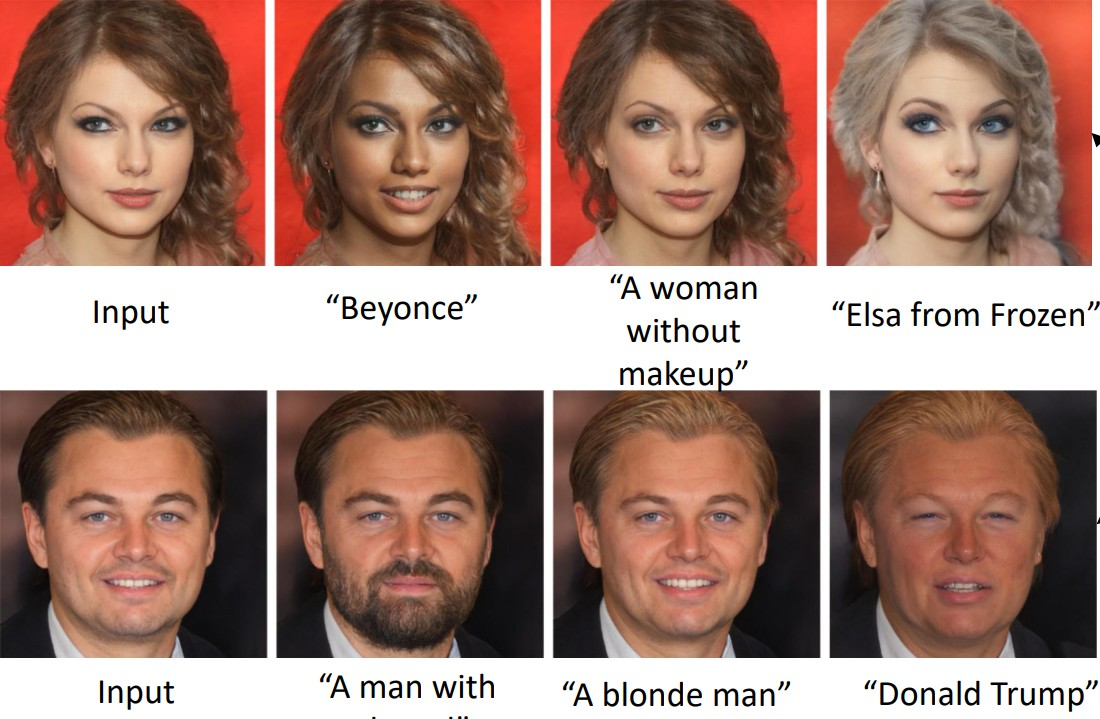
\includegraphics[width=1\textwidth,height=0.9\textheight,keepaspectratio]{images/video/slide_65_1_img.jpg}
    \end{figure}
\framebreak
    \begin{figure}
        \centering
        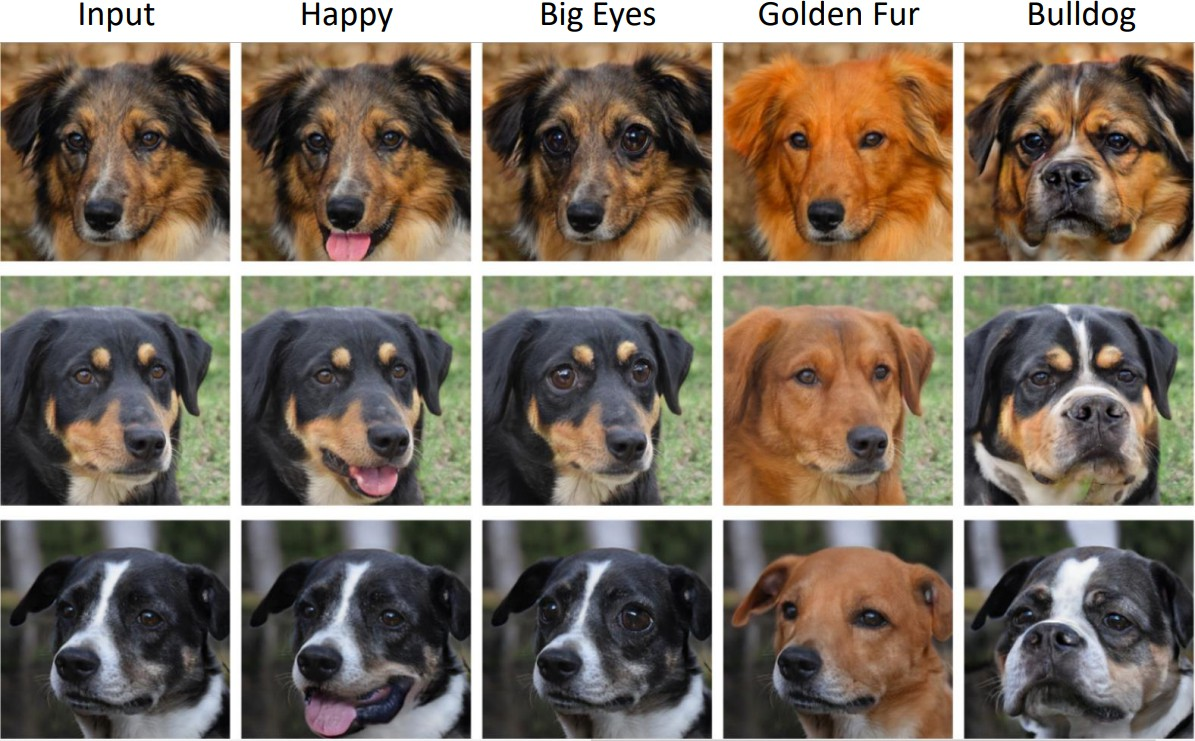
\includegraphics[width=1\textwidth,height=0.9\textheight,keepaspectratio]{images/video/slide_66_1_img.jpg}
    \end{figure}

\framebreak
    \begin{figure}
        \centering
        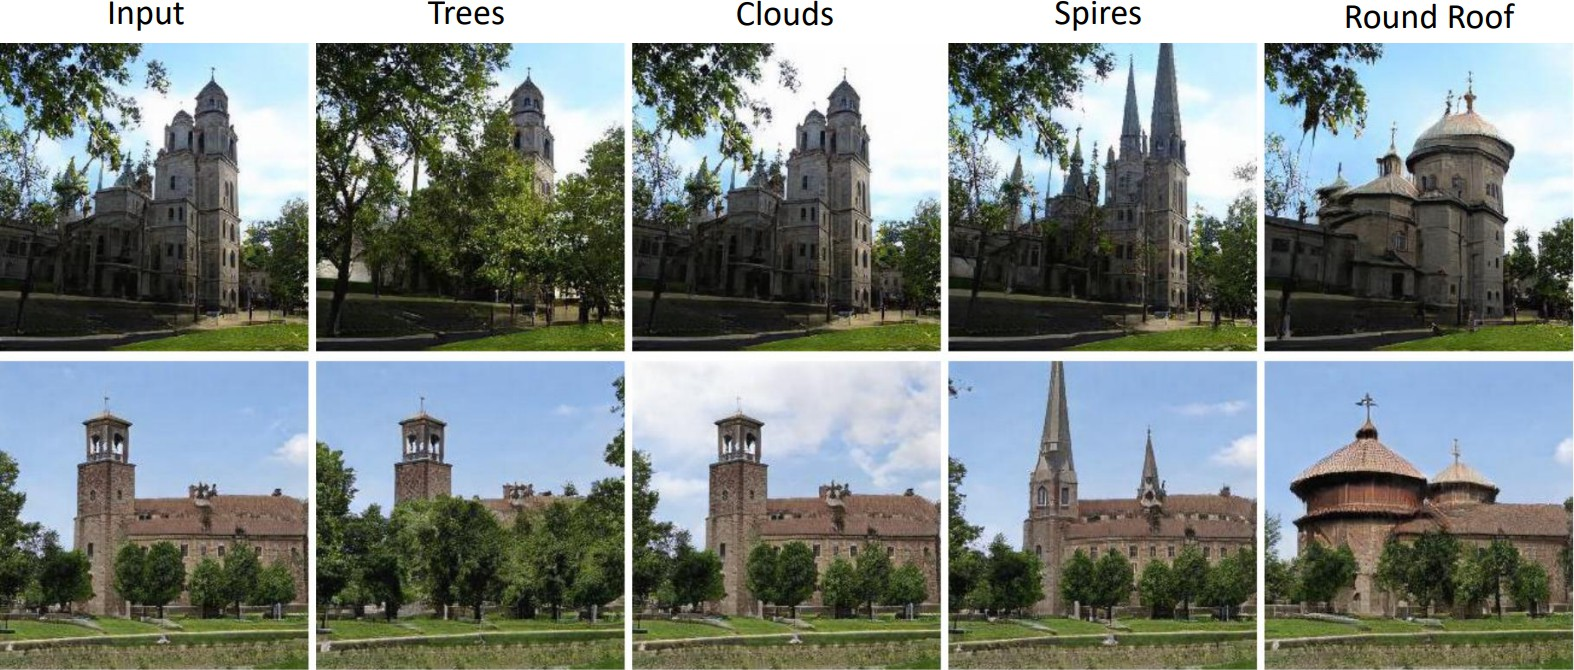
\includegraphics[width=1\textwidth,height=0.9\textheight,keepaspectratio]{images/video/slide_67_1_img.jpg}
    \end{figure}
\end{frame}
\subsection{Text2Live}
\begin{frame}[allowframebreaks]{Text2Live}
    \textbf{Text2Live} is a method that generates live video content from text descriptions, enabling the creation of dynamic and engaging video sequences.

    \begin{itemize}
        \item \textbf{Text-to-Video Generation:} Converts textual descriptions into video sequences, allowing for the synthesis of new video content.
        \item \textbf{Dynamic Content Creation:} Generates videos that can change over time based on the input text, providing a rich visual experience.
        \item \textbf{Applications:} Useful in various domains such as entertainment, education, and marketing, where dynamic video content is required.
    \end{itemize}
\framebreak
    \begin{figure}
        \centering
        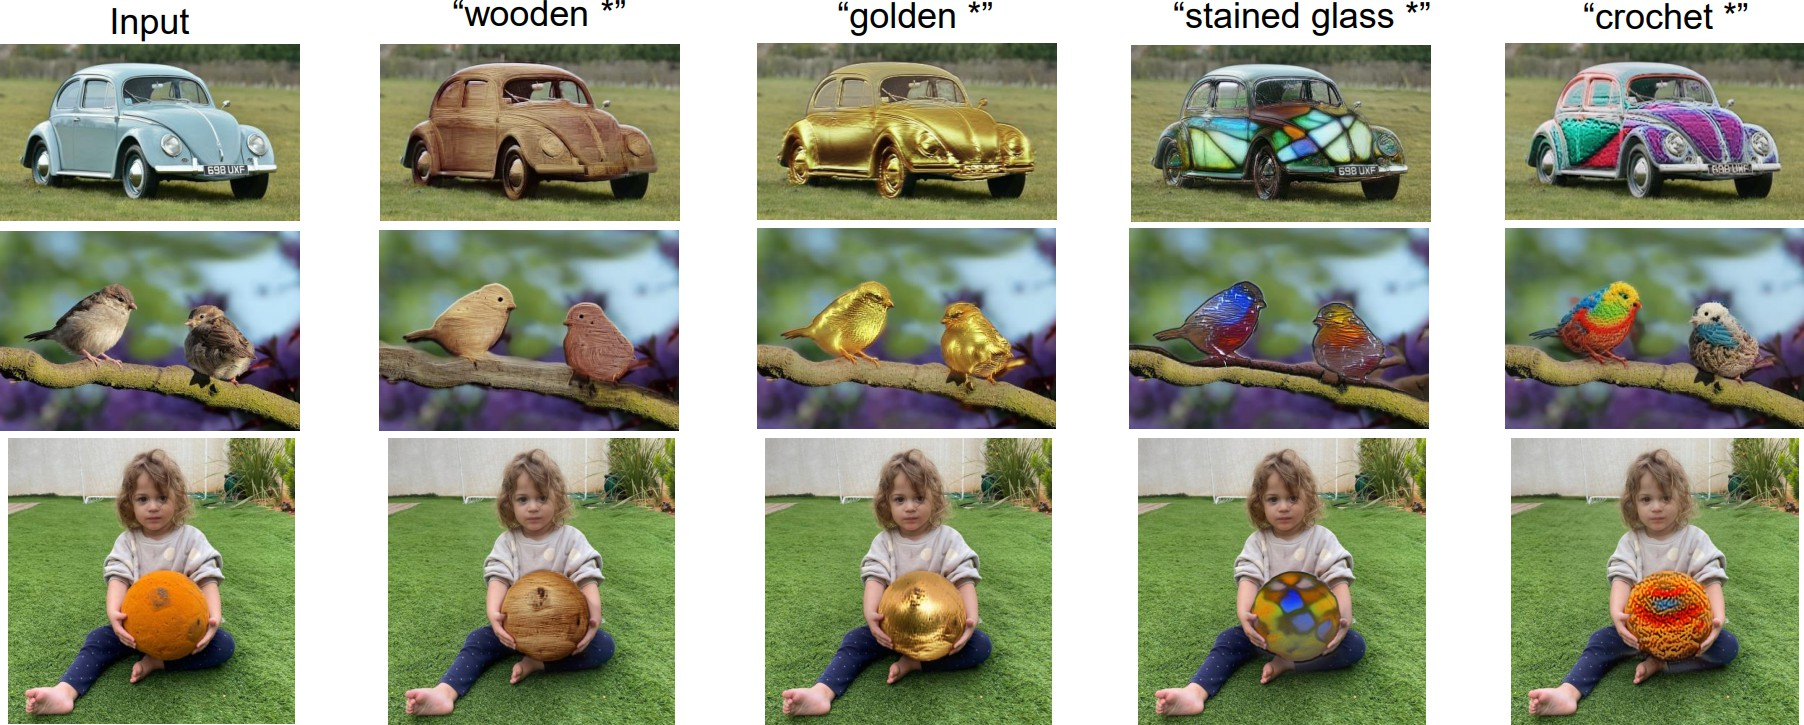
\includegraphics[width=1\textwidth,height=0.8\textheight,keepaspectratio]{images/video/slide_68_1_img.jpg}
    \end{figure}
    {\footnotesize{[Text2LIVE: Text-Driven Layered Image and Video Editing, Bar-Tal Ofri-Amar and Fridman et al. ECCV 2022]}}
\end{frame}
\subsection{Conditional image generation with CLIP Using Diffusion Models}
\begin{frame}[allowframebreaks]{Conditional image generation with CLIP Using Diffusion Models}
    \textbf{Conditional image generation with CLIP Using Diffusion Models} combines the power of diffusion models for image synthesis with CLIP's ability to understand and condition on text prompts, enabling the generation of images that align with specific textual descriptions.

    \begin{itemize}
        \item \textbf{Diffusion Models:} These models generate images by iteratively refining noise into coherent images, allowing for high-quality synthesis.
        \item \textbf{CLIP:} Provides text embeddings that guide the diffusion process, ensuring that the generated images match the desired attributes described in the text.
        \item \textbf{Applications:} Image synthesis, style transfer, and content-aware editing based on textual prompts.
    \end{itemize}
\framebreak
    \begin{figure}
        \centering
        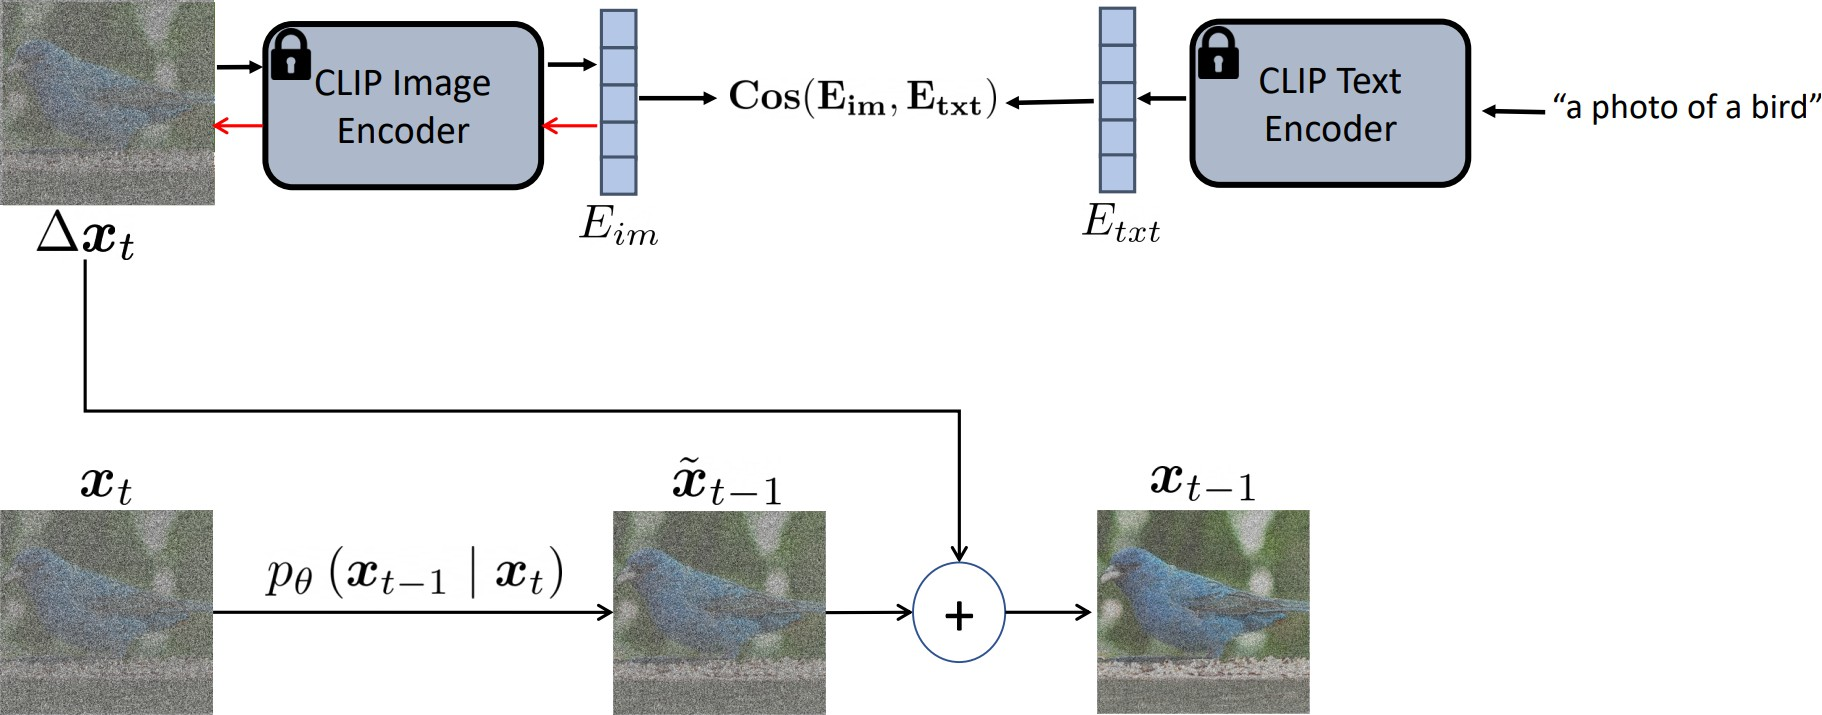
\includegraphics[width=1\textwidth,height=0.8\textheight,keepaspectratio]{images/video/slide_69_1_img.jpg}
    \end{figure}
    {\footnotesize{[Diffusion Models Beat GANs on Image Synthesis, Dhariwal and Nichol et al. NeurIPS 2021]}}
\framebreak
    \begin{figure}
        \centering
        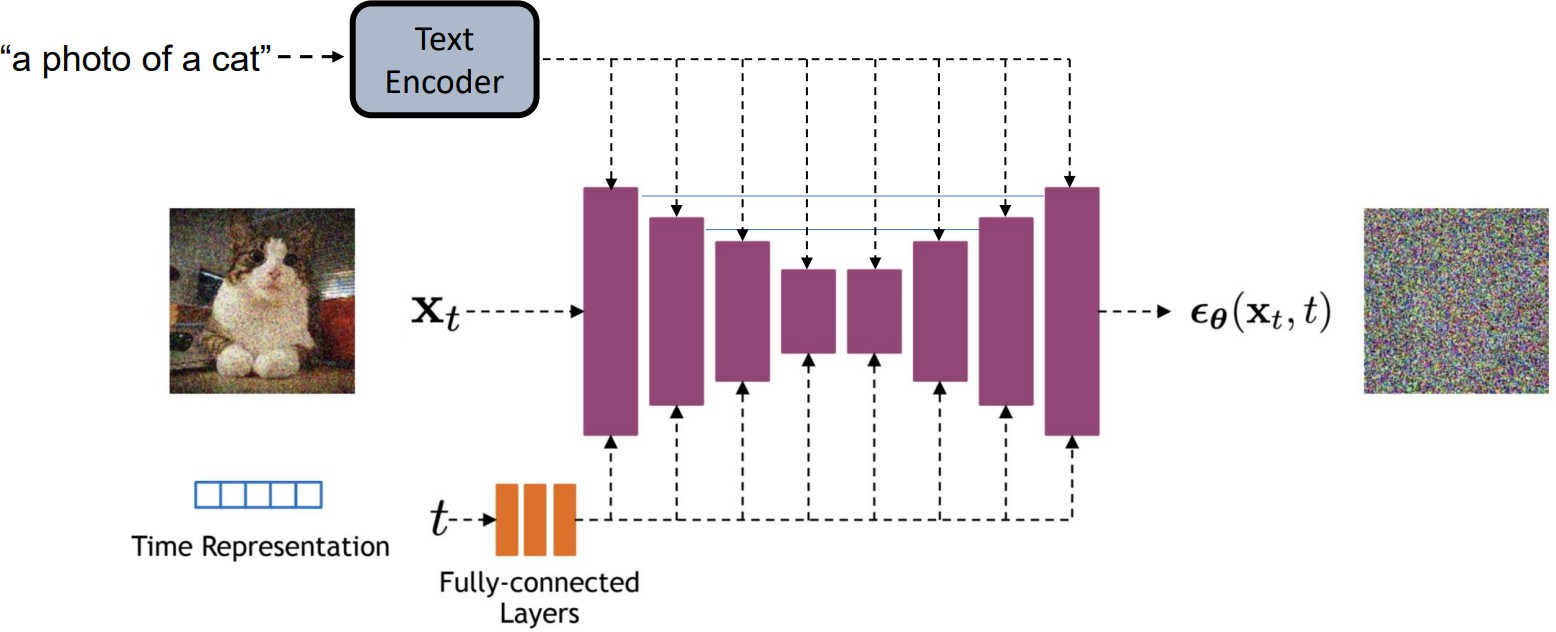
\includegraphics[width=1\textwidth,height=0.9\textheight,keepaspectratio]{images/video/slide_70_1_img.jpg}
    \end{figure}
\end{frame}
\subsection{Text conditioning in Diffusion Models}
\begin{frame}[allowframebreaks]{Text conditioning in Diffusion Models}
    \textbf{Text conditioning in Diffusion Models} enhances the generation of images by incorporating textual descriptions, allowing for more controlled and context-aware image synthesis.

    \begin{itemize}
        \item \textbf{Diffusion Models:} These models generate images by iteratively refining noise into coherent images, enabling high-quality synthesis.
        \item \textbf{Text Conditioning:} Uses text embeddings to guide the diffusion process, ensuring that the generated images align with specific textual descriptions.
        \item \textbf{Applications:} Image synthesis, style transfer, and content-aware editing based on textual prompts.
    \end{itemize}
\framebreak
    \begin{figure}
        \centering
        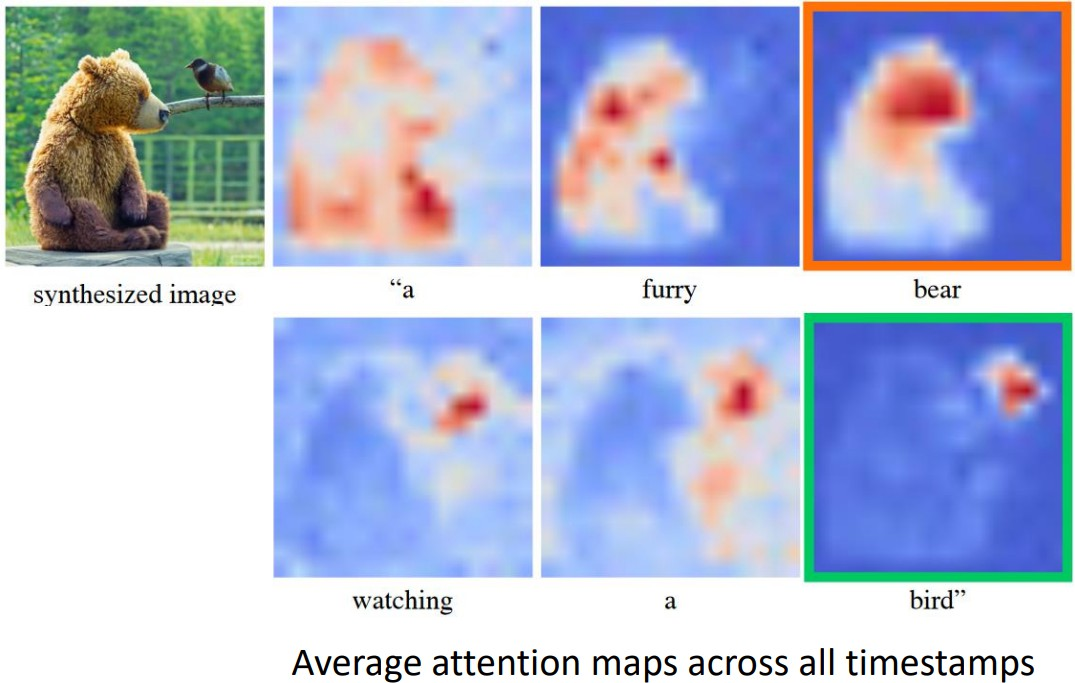
\includegraphics[width=1\textwidth,height=0.8\textheight,keepaspectratio]{images/video/slide_71_1_img.jpg}
    \end{figure}
    {\footnotesize{[Prompt-to-Prompt Image Editing with Cross Attention Control, Hertz and Mokady et al., ICRL 2022]}}
\framebreak
    \begin{figure}
        \centering
        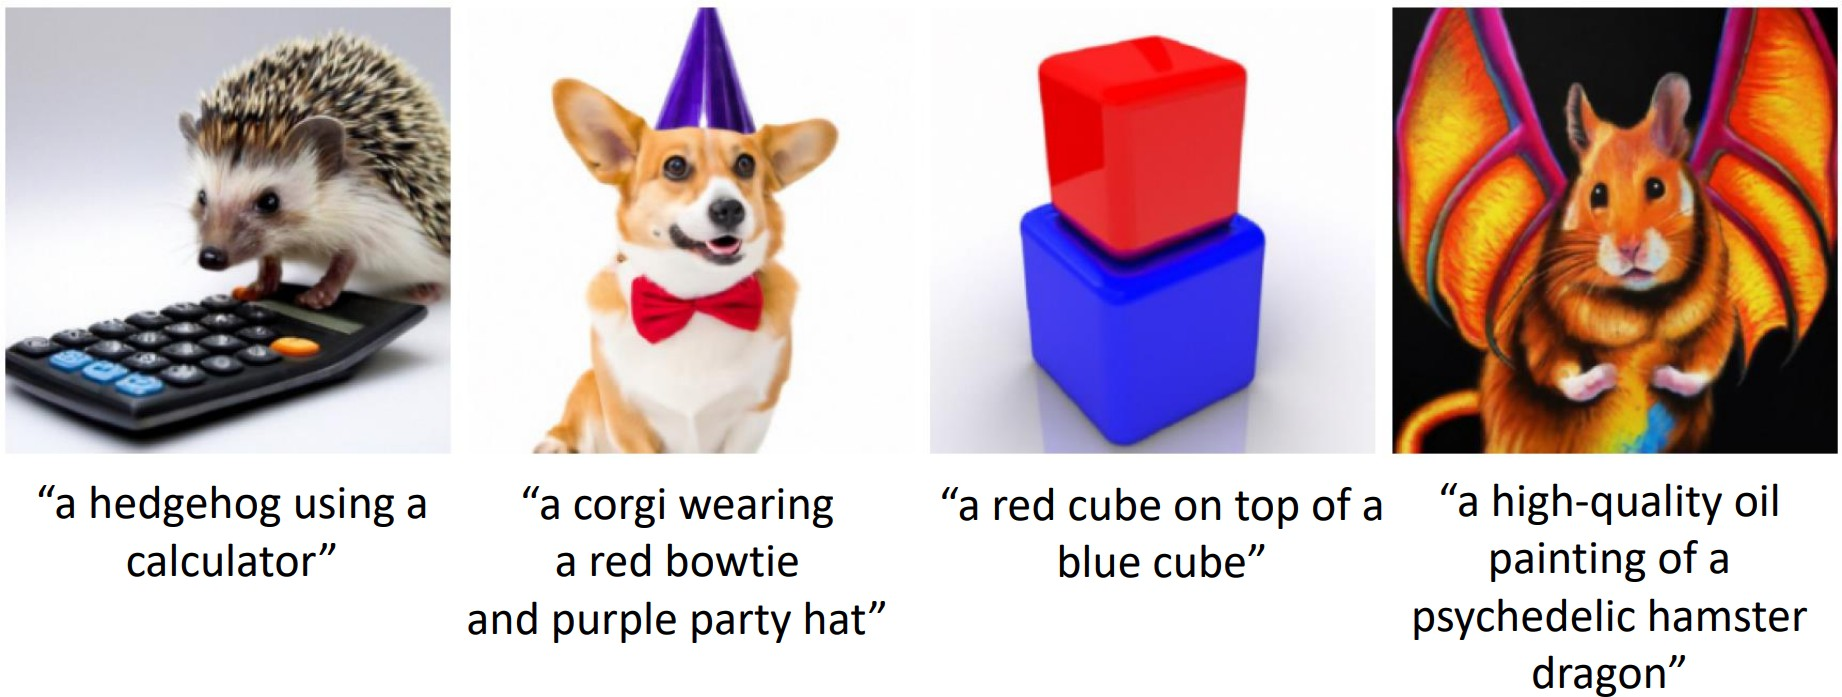
\includegraphics[width=1\textwidth,height=0.9\textheight,keepaspectratio]{images/video/slide_72_1_img.jpg}
    \end{figure}
\end{frame}